\documentclass[10pt]{beamer}

\usetheme[progressbar=foot]{metropolis}
\usepackage{appendixnumberbeamer}
\usepackage{bookmark}
\usepackage{booktabs}
\usepackage[scale=2]{ccicons}

\usepackage{pgfplots}
\usepgfplotslibrary{dateplot}
\pgfplotsset{compat=1.18} 

\usepackage{xspace}
\usepackage{xcolor}

\DeclareMathOperator{\stdev}{stdev}
\DeclareMathOperator{\var}{var}
\DeclareMathOperator{\cov}{cov}
\DeclareMathOperator{\corr}{corr}
\DeclareMathOperator{\prob}{prob}
\DeclareMathOperator{\n}{n}
\DeclareMathOperator{\N}{N}
\DeclareMathOperator{\Cov}{Cov}

\newcommand{\hlf}{\frac{1}{2}}
\newcommand{\bi}{\begin{itemize}}
\newcommand{\ei}{\end{itemize}}
\newcommand{\im}{\item}
\newcommand{\D}{\mathrm{d}}
\newcommand{\E}{\mathrm{e}}
\newcommand{\mye}{\ensuremath{\mathsf{E}}}
\newcommand{\myreal}{\ensuremath{\mathbb{R}}}
\newcommand{\bq}{\begin{equation}}
\newcommand{\eq}{\end{equation}}
\newcommand{\eqdef}{\;\buildrel \text{d{}ef}\over = \;}
\newcommand{\xstar}{\buildrel *\over X}
\newcommand{\pmax}{p^{\text{max}}}
\newcommand{\qmax}{q^{\text{max}}}
\newcommand{\bfr}{\begin{frame}}
\newcommand{\bfrp}{\begin{frame}[plain]}
\newcommand{\efr}{\end{frame}}
\newcommand{\F}{\mathcal{F}}
\newcommand{\FF}{\mathbb{F}}
\newcommand{\ve}{\varepsilon}
\newcommand{\lh}{\hat{\lambda}}
\definecolor{mycolor}{gray}{0.8}
\definecolor{mymaincolor}{rgb}{0.6862745098039216,0.9333333333333333,0.9333333333333333}
\newcommand{\alr}[1]{\textcolor{blue}{#1}}
\definecolor{LightCyan}{rgb}{0.88,1,1}
\newcommand{\yel}{\cellcolor{yellow}}
\newcommand{\blue}{\cellcolor{SkyBlue}}
\newcommand{\gr}{\cellcolor{SpringGreen}}
\newcommand{\pink}{\cellcolor{pink}}
\newcommand{\apr}{\cellcolor{Apricot}}
\newcommand{\tve}{\tilde{\varepsilon}}
\newcommand{\tw}{\tilde{w}}
\newcommand{\ttth}{\tilde{\theta}}
\newcommand{\te}{\tilde{e}}
\newcommand{\ts}{\tilde{s}}
\newcommand{\tx}{\tilde{x}}
\newcommand{\ty}{\tilde{y}}
\newcommand{\tv}{\tilde{v}}
\newcommand{\tp}{\tilde{p}}
\newcommand{\tF}{\tilde{F}}
\newcommand{\tf}{\tilde{f}}
\newcommand{\tZ}{\tilde{Z}}
\newcommand{\ow}{\overline{w}}
\newcommand{\tm}{\tilde{m}}
\newcommand{\tc}{\tilde{c}}
\newcommand{\tz}{\tilde{z}}
\newcommand{\tr}{\widetilde{R}}
\newcommand{\tR}{\widetilde{\mathbf{R}}}
\newcommand{\bms}{\begin{multline*}}
\newcommand{\ems}{\end{multline*}}
\newcommand{\bas}{\begin{align*}}
\newcommand{\eas}{\end{align*}}
\newcommand{\qr}{\mathbb{Q}}
\newcommand{\tX}{\tilde{X}}
\newcommand{\tY}{\tilde{Y}}

\setbeamertemplate{frame footer}{BUSI 521/ECON 505/ECON 505}

\title{Chapter 3: Stochastic Discount Factors}

\date{}
\author{Kerry Back\\ 
BUSI 521/ECON 505\\
Rice University}


\begin{document}

\maketitle



\begin{frame}{Review: First-Order Condition}
 \bi
 \im Assets 1, \ldots, n (including risk-free asset).  Choose $\theta_1, \ldots, \theta_n$ to 
 $$\max \; \mye\left[ u\left( \sum_{i=1}^n \theta_i\tx_i \right) \right] \quad \text{subject to} \quad \sum_{i=1}^n p_i \theta_i = w_0\,.$$
\im Lagrangean:
$$\mye\left[ u\left( \sum_{i=1}^n \theta_i\tx_i \right) \right] - \lambda \left( \sum_{i=1}^n p_i \theta_i - w_0 \right)$$
\im FOC:
$$(\forall \, i) \quad \mye\left[ u'\left( \sum_{i=1}^n \theta_i\tx_i \right) \tx_i \right] = \lambda p_i$$
\im Equivalently,
$$(\forall \, i) \quad \mye\left[ \frac{u'\left( \sum_{i=1}^n \theta_i\tx_i \right) }{\lambda}\tx_i \right] =  p_i$$
\ei
\end{frame}

\begin{frame}{Stochastic Discount Factor}
    \bi 
    \im Definition: A stochastic discount factor (SDF) is any random variable $\tm$ such that
    $$(\forall \, i) \quad \mye\left[ \tm\tx_i \right] =  p_i$$
    \im Or, writing in terms of returns: $\tr_i = \tx_i/p_i$,
    $$(\forall \, i) \quad \mye\left[ \tm\tr_i \right] =  1$$
    \ei 
\end{frame}

\begin{frame}{Risk-Free Asset}
    \bi 
    \im If there is a risk-free asset and $\tm$ is an SDF, then 
    $$\mye[\tm R_f] = 1 \quad \Rightarrow \quad \mye[\tm] = \frac{1}{R_f}$$
    \im Recall that with risk-neutrality, $ m =1/R_f$.
    \im But, with risk aversion, an SDF is stochastic.
    \ei 
\end{frame}

\begin{frame}{Marginal Utility is Proportional to an SDF}
    \bi 
    \im 
    Given the definition of an SDF, we can describe the FOC as: marginal utility is proportional to an SDF; i.e., $u'(\tw^*) = \lambda\tm$.
    \im If there is a risk-free asset, then $\mye[u'(\tw^*)] = \lambda \mye[\tm] = \lambda / R_f$.
    \im So, $\lambda = R_f \mye[u'(\tw^*)]$ and
    $$ \tm = \frac{1}{R_f} \cdot \frac{u'(\tw^*)}{\mye[u'(\tw^*)]}$$
    \im Risk neutrality $\Rightarrow u(w) = a + b w \Rightarrow$
    $$\frac{u'(\tw^*)}{\mye[u'(\tw^*)]} = \frac{b}{b} = 1 \quad \Rightarrow \quad m = \frac{1}{R_f}$$
    \ei 
\end{frame}


\section{Finite State Example}
\subsection{}

\begin{frame}{Example: Finite States}
\bi 
\im
Assume there are $k<\infty$ states of the world. We can regard any random variable as a $k$ vector.  

\im The definition of an SDF $m \in \myreal^k$ is that for each asset payoff $x_i \in \myreal^k$ with price $p_i$ we have
$$p_i \ = \ \sum_{j=1}^k m_jx_{ij} \prob_j $$
\ei
\end{frame}

\begin{frame}{State Prices}
    \bi 
    \im We can set $q_j = m_j\prob_j$ to obtain
$$p_i \ = \ \sum_{j=1}^k x_{ij}q_j$$
\im Definition: An Arrow security is an asset that pays a unit of consumption in a particular state and zero in all other states; i.e., $x = (0 \; \cdots \; 0 \; 1 \; 0 \; \cdots \; 0)^\top$.
\im The price $p$ of an Arrow security equals the $q$ for the state in which it pays 1.  The $q$'s are also called state prices.
\ei 
\end{frame}

\begin{frame}{Example: Equally Probable States}
    \bi
    \im Suppose all states are equally probable.
    \im Assume the FOC holds, so $\tm = u'(\tw^*)/\lambda$ is an SDF.
    \im What can we say about state prices?  Which states are the most expensive and which are the least expensive?
\ei 
\end{frame}


\section{CARA-Normal Example}
\subsection{}

\begin{frame}{CARA Utility}
    \bi 
    \im Suppose there is a CARA investor $u(w) = - \E^{-\alpha w}$.
    \im The FOC gives us 
    $$\tm =  \frac{1}{R_f} \cdot \frac{u'(\tw^*)}{\mye[u'(\tw^*)]} = \frac{1}{R_f} \cdot \frac{\E^{-\alpha \tw^*}}{\mye[\E^{-\alpha \tw^*}]}$$
    \ei
\end{frame}



\begin{frame}{Normal Distributions}
    \bi 
    \im Suppose the asset payoffs $\tx_i$ are joint normally distributed.
    \im $\tw^*$ is a linear combination of the $\tx_i$, so it is joint normal with the $\tx_i$.
   \im The price of each asset is 
   $$p_i = \mye[\tm \tx_i] = \frac{1}{R_f} \cdot \frac{\mye[\E^{-\alpha \tw^*}\tx_i]}{\mye[\E^{-\alpha \tw^*}]}$$
   \im Can we calculate this?
   \ei
\end{frame}


\begin{frame}{Step 1: Project $\tx_i$ on $\tw^*$}
    \bi 
    \im Drop the $i$ subscript and the $^*$ on $\tw^*$.
    \im Setting $b=\cov(\tx,\tw)/\var(\tw)$ and $a=\mye[\tx]-b\mye[\tw]$, we have
    $$\tx = a + b\tw + \te$$
    where $\te$ has a zero mean, and $\te$ and $\tw$ are uncorrelated (easy to check from definitions) and hence independent (by normality).
    \im Thus, $\mye[\E^{-\alpha \tw}\te] = 0$ and
    $$\mye[\E^{-\alpha \tw}\tx] = a\mye[\E^{-\alpha \tw}] + b\mye[\tw \E^{-\alpha \tw}]$$
    $$p = \frac{1}{R_f}\left\{a + b \frac{\mye[\tw \E^{-\alpha \tw}]}{\mye[\E^{-\alpha \tw}]}\right\}$$
    \ei
\end{frame}

\begin{frame}{Step 2: Integrate by Parts}
    \bi
    \im Integrate by parts (using the fact that for the standard normal density $f$, we have $xf(x) = - f'(x)$) or look up in a table of integrals that
    $$\mye[\tw \E^{-\alpha \tw}] = (\mu_w-\alpha \sigma_w^2)\mye[\E^{-\alpha \tw}]$$
    \im We end up with 
    $$p = \frac{a + b \mu_w - \alpha b \sigma_w^2}{R_f}$$
    \im We have $\mye[\tx] = a + b \mu_w$ and $\cov(\tx, \tw) = b\sigma_w^2$, so
    $$p = \frac{\mye[\tx] - \alpha \cov(\tx,\tw)}{R_f}$$
    \ei
    \end{frame}

  
\section{CRRA Example}
\subsection{}

\begin{frame}{CRRA Utility}
    \bi
\im Suppose there is a CRRA investor: $u(w) = w^{1-\rho}/(1-\rho)$.
\im The FOC gives us 
$$\tm =  \frac{1}{R_f} \cdot \frac{u'(\tw^*)}{\mye[u'(\tw^*)]} = \frac{1}{R_f} \cdot \frac{(\tw^*)^{-\rho}}{\mye[(\tw^*)^{-\rho}]}$$
\im The investor's portfolio return is $\tr^*_p := \tw^*/w_0$, so $tw^* = w_0 \tr^*_p$, and we obtain
$$\tm = \frac{1}{R_f} \cdot \frac{(\tr_p^*)^{-\rho}}{\mye[(\tr_p^*)^{-\rho}]}$$
\im More in Chapter 7.
\ei 
\end{frame}

\section{Finite States and Algebra of SDFs}

\begin{frame}{Finite State Model}
\bi 
\im
 $n$ assets and $k$ states.  $X = n \times k$ matrix of asset payoffs.  Each asset is a row.  
\im 
 Vector of asset prices is $p \in \myreal^n$
 \im 
 Portfolio payoff is $X'\theta \in \myreal^k$ for $\theta \in \myreal^n$.  We call $\{X'\theta \mid \theta \in \myreal^n\}$ the span of the assets.
\im 
State price vector is $q \in \myreal^k$ such that $Xq = p$
\im SDF is a vector of state prices divided by probabilities
\ei 
\end{frame}

\begin{frame}{When Does a State Price Vector Exist?}
  \bi \im Assume that if there are two ways of getting the same thing, then they cost the same (Law of One Price):
$$X'\theta = X'\hat{\theta}  \quad \Rightarrow \quad p'\theta = p'\hat{\theta}$$
\im Equivalently, a zero-payoff portfolio must have a zero cost:
$$X'\theta = 0  \quad \Rightarrow \quad p'\theta = 0$$
\im Then an SDF exists.  Proof: if everything orthogonal to the columns of $X$ is also orthogonal to $p$, then $p$ must be a linear combination of the columns of $X$.  This means there exists $q$ such that $Xq = p$.

\ei 
\end{frame}

\begin{frame}{How Many State Price Vectors Are There?}
    \bi
    \im If $q$ is any state price vector and $Xb = 0$ then $q+b$ is a state price vector.  In fact, all state price vectors are $q+b$ where $Xb=0$.  
    \bi 
    \im Proof: Let $\hat{q}$ be another state price vector and define $b=\hat{q} - q$.
    \ei
    \im The dimension of the set of state price vectors is the dimension of the null space of $X$.
    \im There is a unique state price vector if and only if the null space of $X$ is $\{0\}$.  This is equivalent to the rank of $X$ being $k$.
    \im Example: $n=k$ and $X$ nonsingular implies $q = X^{-1}p$.
    \ei 
\end{frame}

\begin{frame}{Complete Markets}
    \bi
    \im We say markets are complete if the span of the assets is all of $\myreal^k$.
    \im Complete markets $\;\Rightarrow\;$ uniqueness of the state price vector.
    \ei
\end{frame}

\begin{frame}{Example}
    \bi \im Two equally probable states of the world.
    \im Risk-free asset with return $R_f=1.1$.  Can take its price to be 1 and its payoff $x$ to be $(1.1, \; 1.1)$.
    \im Single risky asset. Price is 100 and payoffs are $x = (120, \; 90)$. 
    \im So,
    $$p = \begin{pmatrix} 1 \\ 100 \end{pmatrix} \quad \text{and} \quad X = \begin{pmatrix} 1.1 & 1.1 \\ 120 & 190 \end{pmatrix}$$
    \im State price vector solves $Xq = p$, meaning
     \begin{align*}
     1.1q_1  + 1.1q_1 & = 1  \\
    120q_1  + 90q_2 &= 100
    \end{align*}
    \im SDF is $m_1 = 2q_1$, $m_2 = 2 q_2$.  
    \ei
\end{frame}

\begin{frame}{Another Example}
\bi 
\im Two equally probable states.  No risk-free asset.  \im One risky asset with price $p=3$ and payoffs $x = (4, \; 2)$. 
\im State price vector is any $q$ such that $4q_1 + 2q_2 = 3$.
\im SDF is $m_1 = 2q_1$, $m_2=2q_2$, so any $m$ such that $2m_1 + m_2 = 3$.
\ei 
\end{frame}

\begin{frame}
\begin{center}
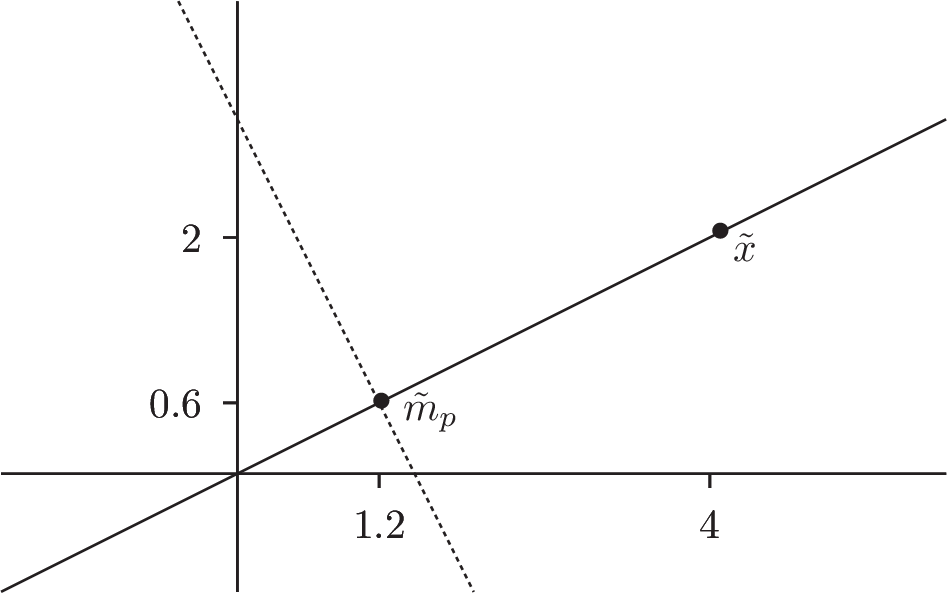
\includegraphics[scale=.7]{images/fig3_2.png}
\end{center}
\bi  \im
The span of the assets is the set $\{(4\theta,\; 2\theta) \mid \theta \in \myreal\}$ and is shown as the solid line.  
\im The set of SDFs is the dotted line.  The intersection of the set of SDFs with the span of the assets is the unique SDF in the span of the assets.  Call it $m_p$ ($p$ for projection). 
\im All SDFs are $m = m_p + y$ where $4y_1 + 2y_2 = 0$.
\ei
\end{frame}

\section{Formulas for Prices and Expected Returns}
\subsection{}


\begin{frame}{Risk Premia as Covariances}
\bi 
\im Because $\cov(\tx,\ty) = \mye[\tx\ty] - \mye[\tx]\mye[\ty]$,
$$1 = \mye[\tm\tr] = \cov(\tm,\tr) + \mye[\tm]\mye[\tr]$$
\im Rearrange to obtain
$$\mye[\tr] = \frac{1}{\mye[\tm]} - \frac{1}{\mye[\tm]}\cov(\tm,\tr)$$
\im Thus, expected asset returns depend on covariances with an SDF.
\im If there is a risk-free asset, then $R_f = 1/\mye[\tm]$.  So,
$$\mye[\tr]-R_f = - R_f\cov(\tm,\tr)$$
\ei
\end{frame}

\begin{frame}{Risk-Adjusted Expected Value}
\bi 
\im 
If there is a risk-free asset, then
$$p \ = \ \mye[\tilde{m}\tilde{x}]  \ = \ \mye[\tilde{m}]\mye[\tilde{x}]+ \cov(\tilde{m},\tilde{x})
\ = \ \frac{\mye[\tilde{x}] + R_f\cov(\tilde{m},\tilde{x})}{R_f}$$
\im So, we can adjust the expected payoff for risk and then discount at the risk-free rate.
\ei 
\end{frame}

\begin{frame}{Risk-Adjusted Discount Rate}
    \bi 
    \im
Also,
\begin{align*}
    \mye[\tr]-R_f = - & R_f\cov(\tm,\tr)\quad 
    \Rightarrow \quad     \mye[\tx/p] = - R_f\cov(\tm,\tr) \\
    &\Rightarrow \quad \mye[\tx]-R_f =p\left[R_f- R_f\cov(\tm,\tr)\right] \\  
     &\Rightarrow \quad p= \frac{\mye[\tilde{x}]}{R_f - R_f\cov(\tilde{m},\tilde{R})}
\end{align*}
\im So we can discount the expected payoff at a risk-adjusted rate. 
\ei 
\end{frame}

\begin{frame}{Risk-Adjusted Probabilities}
\bi 
\im In the finite-state case,
$$p_i = \sum_{j=1}^k m_j x_{ij}\prob_j$$
\im Define
$$\prob^*_j =  \frac{m_j\prob_j}{\sum_j m_j \prob_j} = R_f m_j \prob_j$$
\im Assuming $m>0$, the $\prob^*_j$ are positive, and they sum to 1.  So, we can call them probabilities.
\im Because $m_j\prob_j = \prob^*_j/R_f$, we have
$$p_i = \sum_{j=1}^k m_j x_{ij}\prob_j = \frac{\sum_{j=1}^k x_{ij}\prob^*_j}{R_f} := \frac{\mye^*[\tx]}{R_f}$$
\im So, we can price by taking the expectation with respect to the $\prob^*_j$ and discounting at the risk-free rate.  Consequently, the $\prob^*_j$ are called \alert{risk-neutral probabilities}.
\ei
\end{frame}

\begin{frame}{Example}
    \bi 
    \im Suppose the states are equally probable (under the actual = physical probability) and the FOC holds. 
    \im Which states have higher risk-neutral probabilities?
    \ei
\end{frame}


\begin{frame}{General Definition of Risk-Neutral Probability}
\bi 
\im For an event $A$, set $1_A=\,$ indicator function, meaning $1_A(\omega) = 1$ if $\omega \in A$ and $1_A(\omega) = 0$ otherwise.
\im Given an SDF $\tm$, define 
$$\qr(A) = \frac{ \mye[\tilde{m}1_A]}{\mye[\tm]} = R_f \mye[\tilde{m}1_A]$$
\im Then, $\qr$ is a probability (measure): 
\bi 
\im $\qr(A) \geq 0$, $\qr(\emptyset)=0$, 
\im $\qr(\Omega)=1$, and 
\im $\qr$ of the union of a sequence of disjoint events is the sum of $\qr$ of the events. 
\ei
\ei 
\end{frame}

\begin{frame}{Risk-Neutral Expectation}
    \bi 
\im Let $\mye^*$ denote expectation with respect to $\qr$.  Note $\qr(A) = \mye^*[1_A]$ for all events $A$.  
\im So, the definition of $\qr$ implies
$$(\forall\, A) \quad \mye^*[1_A] = R_f \mye[\tm 1_A]$$

\im This generalizes as
$$(\forall\, \tx) \quad \mye^*[\tx] = R_f \mye[\tm \tx]$$


\im It follows that prices are risk-neutral expected payoffs discounted at the risk-free rate, and risk-neutral expected returns equal the risk-free return: 
$$p = \mye[\tm\tx] = \frac{\mye^*[\tx]}{R_f} \quad \Rightarrow \quad \mye^*[\tilde{R}] \equiv \mye\left[\frac{\tx}{p}\right] = R_f$$
\ei
\end{frame}


\end{document}

\section{Risk Premia}
\subsection{}


\section{RNPs}
\subsection{}

\begin{frame}{Risk Neutral Probabilities}
We can price with an SDF: $p = \mye[\tm\tx]$.

Alternatively, given an SDF, we can ``change probabilities'' to price \alert{as if} investors were risk neutral.  That is, we can price as
$$p \ = \ \frac{\mye^*[\tx]}{R_f}$$
where $\mye^*$ denotes expectation with respect to the changed probabilities.

We call the new probabilities a ``risk-neutral probability'' or ``risk-neutral probability measure.''

\end{frame}

\begin{frame}{Example}
$R_f=1.1$. Single risky asset.  Two states of the world.  $p=100$, $x=120$ or 90 with equal probabilities.

Find the SDF.
\begin{align*}
1  \ & = \ 1.1\prob_1m_1  + 1.1\prob_2m_2  \\
100 \ & = \ 120\prob_1 m_1  + 90\prob_2 m_2
\end{align*}

Find the risk-neutral probability:
\begin{align*}
1  \ & = \ \prob_1^* + \prob_2^*\\
100 \ & = \frac{\ 120 \prob_1^* + 90 \prob_2^*}{1.1} 
\end{align*}

Clearly, $\prob_1^* = 1.1\prob_1 m_1$ and $\prob_2^* = 1.1\prob_2m_2$.
\end{frame}

\begin{frame}{Example cont.}
Let's price another asset in the example.  Consider a security that pays \$1 if $x=120$ and 0 otherwise.  

Price using SDF: ???
\vskip 3\baselineskip
Price using RNP: ???
\end{frame}

\begin{frame}{General Definition of RNP}
For an event $A$, $1_A=\,$ indicator function, meaning $1_A(\omega) = 1$ if $\omega \in A$ and $1_A(\omega) = 0$ otherwise.

Given an SDF $\tm$, define 
$$\qr(A) = \frac{ \mye[\tilde{m}1_A]}{\mye[\tm]} = R_f \mye[\tilde{m}1_A]$$

Then, $\qr$ is a probability: $\qr(A) \geq 0$, $\qr(\emptyset)=0$, $\qr(\Omega)=1$, and $\qr$ of the union of a sequence of disjoint events is the sum of $\qr$ of the events.

In the example: \vspace*{-\baselineskip}
\begin{itemize}
    \item For $A=\{\tx=120\}$,
$\qr(A) \eqdef \prob_1^* = 1.1 \prob_1 m_1$.
\item For $A = \{\tx=90\}$,
$\qr(A) \eqdef \prob_2^* = 1.1 \prob_2 m_2$.
\end{itemize}


\end{frame}


\begin{frame}{Risk-Neutral Expectation}
Let $\mye^*$ denote expectation with respect to $\qr$.  Note $\qr(A) = \mye^*[1_A]$ for all events $A$.  

So, the definition of $\qr$ implies
$$(\forall\, A) \quad \mye^*[1_A] = R_f \mye[\tm 1_A]$$

This generalizes as
$$(\forall\, \tx) \quad \mye^*[\tx] = R_f \mye[\tm \tx]$$


It follows that \alert{prices are risk-neutral expected payoffs discounted at the risk-free rate, and risk-neutral expected returns equal the risk-free return}: 
$$p = \mye[\tm\tx] = \frac{\mye^*[\tx]}{R_f} \quad \Rightarrow \quad \mye^*[\tilde{R}] = \frac{\mye^*[\tx]}{p} = R_f$$

\end{frame}


\end{document}